Das Grammatical Framework ist ein Softwaresystem mit einer spezialisierten Programmiersprache zur Entwicklung von Grammatiken. Es benutzt Formalismen, wie sie auch in modernen funktionalen Programmiersprachen wie Haskell zu finden sind, unterstützt aber vor allem die Entwicklung von Anwendungen zur Verarbeitung natürlicher Sprachen.\footnote{vgl. \cite{RANTA2011} S. vii} Somit können einem manche Konzepte bereits vertraut sein, wenn man sich schon mit den Möglichkeiten der funktionalen Programmierung\footnote{Beispiele für funktionale Programmiersprachen sind Lisp, SML und Haskell} auseinander gesetzt hat. Ein großer Vorteil des Grammatical Frameworks im Vergleich zu anderen Parsingsystemen ist, dass durch das Typsystem, das unter anderem auf der Typtheorie von Martin-Löf basiert, Grammatikfehler schon durch den Compiler erkannt werden können.\footnote{vgl. \cite{RANTA2011} S. 127ff.} \par
Die große Stärke des Grammatical Frameworks ist die Multilingualität. Das Grundkonzept für die Unterstützung verschiedener Sprachen ist die Trennung in eine konkrete und eine abstrakte Repräsentation der Grammatik. Dabei haben die unterschiedlichen Sprachen eine gemeinsame abstrakte Struktur. Die konkrete Syntax dagegen beschreibt, wie aus einer sprachunabhängigen Repräsentation eines "`Satzes"' eine für die jeweilige Sprache spezifische Zeichenkette erzeugt werden kann. Über diesen Schritt der abstrakten Repräsentation kann man eine Übersetzung zwischen verschiedensten Sprachen umsetzen, die eine gemeinsame abstrakte Syntax teilen.\footnote{vgl. \cite{RANTA2011} S. 10ff.} Die Details dieses Formalismus sollen nun an einigen kleinen deutsch-englischen Beispielen genauer betrachtet werden.
\pagebreak
\subsection{Der Grammatikformalismus}
\label{subsec:grammatik}
Im Bereich der Computerlinguistik und Informatik werden hauptsächlich kontextfreie Grammatiken, also Grammatiken von Typ 2 der Chomsky-Hierarchie, verwendet.\footnote{vgl. \cite{SCHOENING2008} S. 9f} Die zwei Hauptgründe dafür sind, dass die Mächtigkeit dieses Formalismuses meist ausreicht, die gewünschten Sprachen zu beschreiben. So sind in kontextfreien Sprachen geklammerte Ausdrücke möglich, die bei Programmiersprachen recht häufig sind.\footnote{vgl. \cite{SCHOENING2008} S. 43} Zudem ist der Verarbeitungsaufwand gering im Vergleich zu Grammatiken einer der höheren Stufen, und es existieren effiziente Algorithmen zum Parsen mit kontextfreien Grammatiken, so z.B. der Cocke-Younger-Kasami-Algorithmus, auch bekannt als CYK-Algorithmus.\footnote{vgl. \cite{SCHOENING2008} S. 56f.}
\begin{program}[h!tp]
\begin{tabular}{llll}
1 & S & $\longrightarrow$ & NP, VP \\
2 & NP & $\longrightarrow$ & Det, N \\
3 & N & $\longrightarrow$ & \textit{Mann} \\
4 & Det & $\longrightarrow$ & \textit{der} \\
5 & VP & $\longrightarrow$ & V \\
6 & V  & $\longrightarrow$ & \textit{schläft} \\
\end{tabular}
\caption{Kurzes Beispiel einer kontextfreien Grammatik}
\label{CFG-Beispiel}
\end{program}
Die in Beispiel \ref{CFG-Beispiel} gegebene Grammatik ist ein sehr minimalistisches Beispiel für eine kontextfreie Grammatik. Mit ihrer Hilfe kann nur der eine deutsche Satz "`Der Mann schläft"' hergeleitet werden. Eine mögliche Ableitung hat die in Beispiel \ref{CFG-Ableitung} gezeigte Form. Bei dieser Ableitung wurde top-down vorgegangen, also von der allgemeinsten Kategorie hinab bis zur spezifischen Zeichenkette. Alternativ wäre es auch möglich gewesen, eine bottom-up-Ableitung anzugeben, die lediglich dem Ablesen der gegebenen Ableitung von unten nach oben entspricht. In der Grammatik sind die Regeln zum einfacheren Bezug auf die Grammatik mit Regelnummern versehen. Diese Regelnummern sind deshalb auch in der Ableitung und dem entsprechenden Syntaxbaum zu sehen. \par
\begin{program}[h!tp]
\begin{Verbatim}[commandchars=\\\{\},codes={\catcode`$=3\catcode`^=7}] 
                    S
                    $\overset{1}{\Rightarrow}$ NP VP
                    $\overset{2}{\Rightarrow}$ Det N VP
                    $\overset{4}{\Rightarrow}$ \textit{der} N VP
                    $\overset{3}{\Rightarrow}$ \textit{der Mann} VP
                    $\overset{5}{\Rightarrow}$ \textit{der Mann} V
                    $\overset{6}{\Rightarrow}$ \textit{der Mann schläft}
\end{Verbatim}
\caption{Ableitung des Satzes mit Hilfe der Grammatik aus Beispiel \ref{CFG-Beispiel}}
\label{CFG-Ableitung}
\end{program}
% $ Just to fix errors in syntax highlighting
\begin{figure}[h!tp]
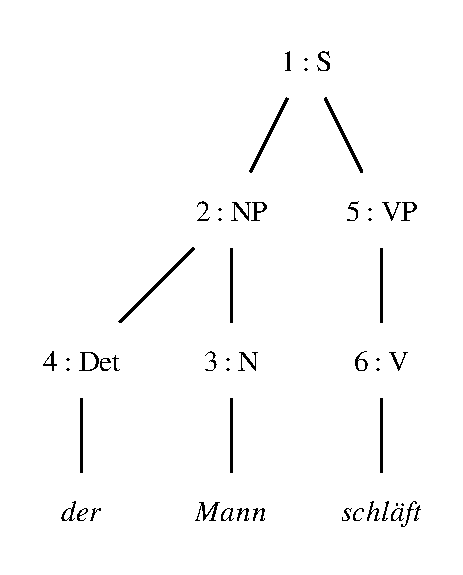
\includegraphics{graphics/MiniSatzSyntax.eps}
\caption{Syntaxbaum für die Ableitung in Beispiel \ref{CFG-Ableitung}}
\label{CFG-Syntaxbaum}
\end{figure}
Im Formalismus des Grammatical Framework wird die oben gegebene Grammatik in eine abstrakte und eine konkrete Syntax zerlegt. So entspricht diese abstrakte Syntax in etwa dem Syntaxbaum in Abbildung \ref{CFG-Syntaxbaum} ohne die terminalen Blätter. \par
% Listing MiniSatzAbs
\lstinputlisting[float=h!tp,caption={Abstrakte Syntax der Grammatik aus Beispiel \ref{CFG-Beispiel}},label={GF-MiniSatzAbs}]{minisatz/MiniSatzAbs.gf}
Die abstrakte Syntax der kontextfreien Grammatik aus Beispiel \ref{CFG-Beispiel} ist in Listing \ref{GF-MiniSatzAbs} zu sehen. Zunächst gibt das Schlüsselwort \texttt{abstract} an, dass es sich um eine Datei mit einer abstrakten Syntaxbeschreibung handelt. Diesem Schlüsselwort folgt der Name und nach dem \texttt{=} der Inhalt der Grammatik. \par
Zuerst werden mit Hilfe der \texttt{flags}-Direktive einige mögliche Einstellungen vorgenommen. In diesem sehr kurzen Beispiel wird nur die Startkategorie für das Parsing gesetzt, also die Wurzel aller Parsebäume. Andere mögliche Optionen sind z.B. die Einstellungen des Encodings und der Lexer, also das Programm, das die Eingabe in lexikalische Tokens zerlegt.\footnote{vgl. \cite{RANTA2011} S. 54f.} \par
Nach dem Schlüsselwort \texttt{cat} folgt eine Liste der Kategorien oder auch Non-Terminal-Symbole. Sie entsprechen Datentypdefinition in (funktionalen) Programmiersprachen. \par
Hauptbestandteil der Grammatik sind die Syntaxregeln. Sie werden nach dem Schlüsselwort \texttt{fun} aufgelistet. Die Regeln ähneln der Form von Funktionssignaturen in Sprachen wie Standard ML oder Haskell, denn sie beschreiben lediglich die Bestandteile, aus denen ein Ausdruck einer neuen Kategorie zusammengesetzt werden soll. Das genaue Vorgehen für die Kombination dieser Bestandteile wird dann sprachspezifisch in jeder konkreten Grammatik, die diese abstrakte Grammatik implementiert, beschrieben. So sagt die erste Regel mit dem Namen \texttt{mkNP} aus, dass ein Ausdruck der Kategorie \texttt{NP} aus einem Ausdruck der Kategorie \texttt{Det} und aus einem Ausdruck der Kategorie \texttt{N} zusammengesetzt werden kann. Dabei ist aber noch keine Aussage über die endgültige Reihenfolge der Bestandteile in konkreten Zeichenketten getroffen. Die letzten drei Regeln führen lediglich die lexikalische Einheiten mit einer entsprechenden Kategorie ein. \par
Diese abstrakte Grammatik kann nun konkret umgesetzt werden. Zwei konkrete Implementierungen, für Deutsch und Englisch, sind in Listing \ref{GF-MiniSatzGer} und \ref{GF-MiniSatzEng} zu finden. \par
% Listing MiniSatzGer
\lstinputlisting[float=h!tp,caption={Konkrete deutsche Syntax für die abstrakte Syntax in Listing \ref{GF-MiniSatzAbs}},label={GF-MiniSatzGer}]{minisatz/MiniSatzGer.gf}
% Listing MiniSatzEng
\lstinputlisting[float=h!tp,caption={Konkrete englische Syntax für die abstrakte Syntax in Listing \ref{GF-MiniSatzAbs}},label={GF-MiniSatzEng}]{minisatz/MiniSatzEng.gf}
Zunächst weist das Schlüsselwort \texttt{concrete} die Grammatik als eine konkrete Grammatik aus. Es folgt wie bei einer abstrakten Syntax der Name der Grammatik, diesmal wird jedoch darauf folgend angegeben, welche abstrakte Grammatik die Grundlage bietet, hier unsere \texttt{MiniSatzAbs}-Grammatik. \par
Das in der deutschen, konkreten Grammatik verwendete Flag \texttt{coding} ermöglicht es, die Zeichenkodierung in den Zeichenketten festzulegen. In diesem Falle ist es für die deutschen Umlaute nötig, die Zeichenkodierung anzugeben. Für andere Sprachen mit komplett vom lateinischen unterschiedlichen Schriftsystemen gibt es auch die Möglichkeit, statt der direkten Zeichenkodierung eine Transliteration zu verwenden. Dafür wird eine bijektive Abbildung zwischen Unicode-Zeichen und Zeichenketten der Länge eins oder größer, die nur aus ASCII-Zeichen bestehen, verwendet.\footnote{vgl. \cite{RANTA2011} S. 55 und S. 227f.} \par
Das Schlüsselwort \texttt{lincat} ist die konkrete Entsprechung zum Schlüsselwort \texttt{cat} in der abstrakten Syntax. Hier muss für jede in der abstrakten Syntax angegebene Kategorie ein konkreter Datentyp angegeben werden. In diesem Falle wurde für alle Kategorien der einfache Datentyp \texttt{Str}, also eine einfache Zeichenkette\footnote{Um genau zu sein, eine Liste von Token, die bei der Linearisierung mit Leerzeichen konkateniert werden}, gewählt. Das Grammatical Framework unterstützt auch verschiedene Arten komplexer Datentypen, die später näher erläutert werden. \par
Auf den \texttt{lincat}-Block folgt, mit dem Schlüsselwort \texttt{lin} markiert, der Abschnitt, in dem die für jede abstrakte Syntaxregel beschrieben wird, wie diese in eine konkrete Zeichenkette zu übersetzen ist. Für die drei lexikalischen Regeln \texttt{Mann\_N}, \texttt{der\_Det} und \texttt{schlafen\_N} ist dies lediglich die entsprechende Zeichenkette z.B. für \texttt{Mann\_N} "`Mann"' im Deutschen bzw. "`man"' im Englischen. Die restlichen Syntaxregeln sind in diesem Beispiel nur geringfügig komplexer. Die Regel \texttt{mkVP} gibt lediglich den Parameter als Rückgabewert zurück, bildet also die gleiche Zeichenkette, der bereits als Parameter übergeben wurde. Und die beiden verbleibenden Regeln \texttt{mkNP} und \texttt{mkS} konkatenieren einfach mit Hilfe des Operators \texttt{++} die beiden als Parameter übergebenen Zeichenketten. \par
Man kann diese sehr kurzen konkreten Grammatiken zusammen mit der gemeinsamen Grammatik in das Grammatical Framework laden und in einer der beiden Sprachen den Satz "`der Mann schläft"' bzw. "`the man sleeps"' parsen und die so erhaltene abstrakte Repräsentation \texttt{(mkS (mkNP der\_Det Mann\_N) (mkVP schlafen\_V))} in die andere Sprache linearisieren, also mit Hilfe der konkreten Syntaxregeln die entsprechende Zeichenkette in der Sprache generieren. \par
\begin{figure}
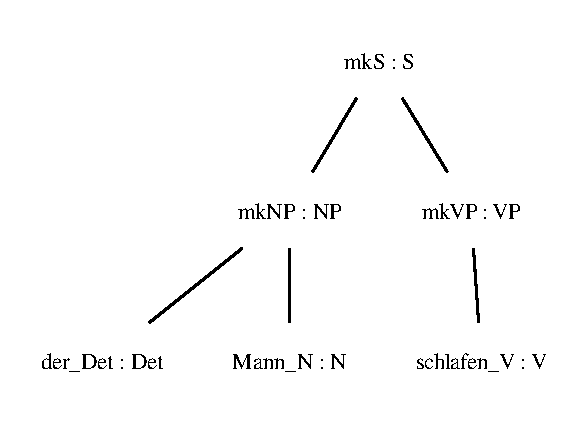
\includegraphics{graphics/MiniSatzTree.eps}
\caption{Baum der abstrakten Syntax für den Satz "`der Mann schläft"'}\label{MiniSatz-AbsTree}
\end{figure}
\begin{figure}
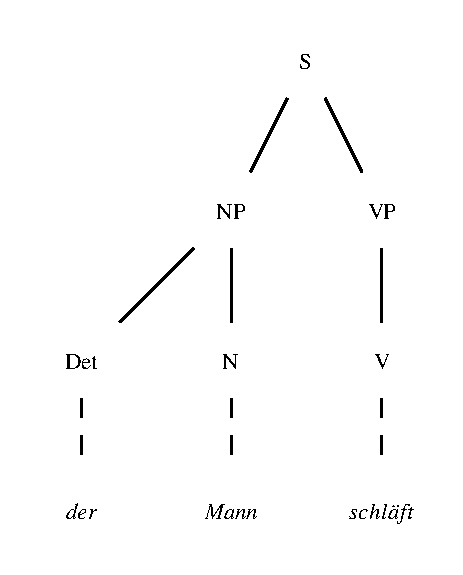
\includegraphics{graphics/MiniSatzParseGer.eps}
\caption{Parsebaum der konkreten deutschen Syntax}\label{MiniSatz-ParseGer}
\end{figure}
Mit Hilfe des Grammatical Frameworks kann man sich sowohl den abstrakten Syntaxbaum und als auch den konkreten Parsebaum für eine der implementierten Sprachen grafisch darstellen lassen. Diese Bäume für die MiniSatz-Grammatik sind in Abb. \ref{MiniSatz-AbsTree} und \ref{MiniSatz-ParseGer} zu sehen. \par
% Listing SatzAbs
\lstinputlisting[float=h!tp,caption={Aus Listing \ref{GF-MiniSatzAbs} erweiterte abstrakte Syntax \texttt{SatzAbs}},label={GF-SatzAbs}]{satz/SatzAbs.gf}
Nun kann man diese doch sehr minimalistische Grammatik etwas erweitern, so dass man auch die Sätze "`die Frauen schlafen"', "`der Mann sieht die Frau"' und "`der Mann liest das Buch"' erkennen kann. Die fertigen Quelltextdateien sind in Listing \ref{GF-SatzAbs}, \ref{GF-SatzGer} und \ref{GF-SatzEng} zu finden. Die Veränderungen in der abstrakten Syntax (Listing \ref{GF-SatzAbs}) betreffen hauptsächlich die Einführung von transitiven Verben mit der Kategorie \texttt{V2}. Mit der Funktion \texttt{mkVP2} wird aus einem transitiven Verb und einer Nominalphrase eine Verbalphrase mit Akkusativobjekt aufgebaut. Um auch Nominalphrasen im Plural zu ermöglichen, wird für den bestimmten Artikel eine Singular- und eine Pluralform benötigt. Auch das "`Lexikon"', also die Liste der lexikalischen Einheiten, wird um die Wörter für "`Frau"', "`Buch"', "`sehen"' und "`lesen"' erweitert. \par
% Listing SatzGer
\lstinputlisting[float=h!tp,caption={Erweiterte konkrete deutsche Syntax  \texttt{SatzGer}},label={GF-SatzGer},basicstyle=\footnotesize]{satz/SatzGer.gf}
In der konkreten Umsetzung sind nun aber größere Unterschiede, sowohl zur ursprünglichen Grammatik, als auch zwischen den unterschiedlichen Sprachen zu finden. Bei der konkreten deutschen Grammatik werden zuerst nach dem Schlüsselwort \texttt{param} drei neue Datentypen dadurch definiert, dass ihr Wertebereich aufgezählt wird. So wird definiert, dass im Deutschen der Genus die drei Werte Maskulin, Feminin, und Neutrum annehmen kann, der Numerus die Werte Singular und Plural und in diesem Beispiel Kasus die zwei Werte Nominativ und Akkusativ. Alle weiteren Fälle werden in diesem kleinen Beispiel nicht benötigt. Die nächste größere Änderung ist im \texttt{lincat}-Block zu finden. Denn statt allen Kategorien den selben einfachen Datentyp zu geben, haben nun alle Kategorien einen komplexen Typ. Zunächst sind all diese Typen Verbundtypen, in Englisch Records, zu erkennen an den geschweiften Klammern. Sie sammeln Objekte\footnote{Der Begriff Objekt wird, obwohl es sich bei dem Grammatical Framework nicht um eine objekt-orientierte Programmiersprache handelt, für Konstrukte eines bestimmten Typs verwendet} möglicherweise verschiedenen Typs in einem einzigen Objekt zusammen. Jedes dieser inneren Objekte hat einen Typ und einen Bezeichner, über den darauf zugegriffen werden kann.\footnote{Verbundtypen haben die Form \texttt{\{$l_1 : T_1 ; \dots ; l_n : T_n$\}} mit $l_1, \dots, l_n$ endlich viele verschiedenen Bezeichnern und $T_1, \dots, T_n$ beliebige Typen. Objekte dieser Typen haben die Form \texttt{\{$l_1 = v_1 ; \dots ; l_n = v_n$\}} mit $v_i$ Werte vom Typ $T_i$ für jedes $i$ mit $1\leq i\leq n$ (vgl. \cite{RANTA2011} S. 279)} Auf diese Weise haben z.B. Nomen ein inhärentes Genus, gespeichert im Bezeichner \texttt{g}, und eine Form, die hier nur vom Numerus abhängig ist, gespeichert im Bezeichner \texttt{s}. Üblicherweise ist die Nomenform auch vom Kasus abhängig, allerdings betrachten wir nur die beiden Kasus Nominativ und Akkusativ, bei denen hier die Nomen immer die selbe Form bilden. Nach diesem Schema sind die Typen für alle Kategorien aufgebaut. Um die Abhängigkeit eines Wertes von gewissen anderen Werten auszudrücken, gibt es im Grammatical Framework die so genannten Tabellentypen\footnote{Tabellentypen haben die Form \texttt{\{$Typ_1$ => $Typ_2$\}} mit $Typ_1,Typ,2$ beliebige Typen und Tabellenobjekte die Form \texttt{table \{ $k_1 => V_1 ; \dots ; k_n => V_n$ \}} mit $k_i$ von $Typ_1$ und $V_i$ vom $Typ_2$ (Tabellentypen sind im Grammatical Framework Sonderfälle von Funktionen, weswegen in dieser Arbeit nicht genauer auf die Funktionsweise eingegangen werden soll. Details sind bei \cite{RANTA2011} S. 281f. zu finden)}, wie sie auch bei den \texttt{s}-Feldern von \textit{Det}, \textit{N}, \textit{NP}, etc. zu sehen ist. Dies bedeutet, dass der Wert aus dem Bereich von $Typ_2$ vom Wert aus dem Bereich $Typ_1$ abhängt.\footnote{vgl. \cite{RANTA2011} S. 59} \par
Um es noch einmal zusammenzufassen, die Typen für die Kategorien im \texttt{licat}-""Bereich sind nun statt des einfachen Typs \texttt{Str} Verbundtypen, bestehend aus mehreren Objekten, deren Werte wiederum von anderen Werten abhängig sein können. Wie das konkret funktioniert, wird im nächsten Abschnitt sichtbar. Denn es müssen sowohl für die Verbundtypen als auch für die Tabellentypen konkrete Objekte erzeugt werden. Dies geschieht im \texttt{lin}-Block, in dem nun die konkreten Grammatikregeln "`konstruiert"' werden. Fangen wir am besten von hinten, also von den lexikalischen Regeln her, an. Der Typ für Verben, ungeachtet ob es transitive, also \texttt{V2}-Verben, oder intransitive \texttt{V}-Verben sind, gibt an, dass sie aus einem einzigen Tabellenobjekt mit dem Bezeichner \texttt{s} bestehen. Diese Tabelle hat den Typ \texttt{Numerus => Str}, also eine \texttt{Str}-Zeichenkette, deren Wert von einem Numerus abhängt. Üblicherweise enthält das \texttt{s}-Feld in Grammatiken des Grammatical Framework das Paradigma, also eine Tabelle, die alle Wortformen enthält. So ein Verbund wird jeweils für die Verben \texttt{lesen\_V2}, \texttt{sehen\_V2} und \texttt{schlafen\_V} konstruiert. Die geschweiften Klammern geben wieder an, dass es sich um einen Verbund handelt, der als Wert erzeugt werden soll. Dann folgt der Bezeichner \texttt{s} dem mit dem Zuweisungsoperator \texttt{=} ein Wert zugewiesen werden soll. Dieser Wert wiederum soll eine Tabelle des genannten Typs sein. Diese wird mit dem Schlüsselwort \texttt{table} erzeugt. In den darauf folgenden geschweiften Klammern muss nun jedem möglichen Wert des Datentyps, in diesem Falle \texttt{Numerus}, ein Wert des abhängigen Typs, hier \texttt{Str}, zugeordnet werden. Dazu wird der Operator \texttt{=>} verwendet. Der Typ \texttt{Numerus} hat die zwei Werte \texttt{Sg} und \texttt{Pl} und die Verben haben in dieser Grammatik zwei Formen. Verben hier nur in zwei Formen vor, der 3. Person-Präsens-Indikativ-Singular- und 3.-Person-Präsens-Indikativ-Plural-Form. So hat das Verb \texttt{lesen\_V} die folgenden zwei Formen "`liest"' und "`lesen"'. \par
Nach dem selben Schema funktionieren auch die restlichen Verben und die Nomen. Allerdings haben die Nomen ihr inhärentes Genus. Deshalb haben sie in ihrem Verbund zusätzlich den Bezeichner \texttt{g}, dem das grammatische Geschlecht des Nomens in der lexikalischen Regel \texttt{Mann\_N}, \texttt{Frau\_N} und \texttt{Buch\_N} zugewiesen wird. Es ist recht offensichtlich, dass \texttt{Mann\_N} maskulin, \texttt{Frau\_N} feminin und \texttt{Buch\_N} neutral sein sollte. \par
Gegenüber dem Typ der Nomen und Verben ist der Typ des Determinans, in diesem Falle der bestimmte Artikel, im Singular etwas komplizierter. Die Artikel haben ein inhärentes Numerusmerkmal, das den Numerus des Nomens in der Nominalphrase regiert. Deshalb gibt es für Singular- und Pluralartikel je eine eigene Regel. \par 
Die Form des Artikels ist sowohl von Genus als auch von Kasus abhängig. Deshalb wird dem \texttt{s}-Feld bei \texttt{defArtSg\_Det} eine Tabelle zugewiesen, in der jedem Wert für Genus erneut eine Tabelle über die Werte des Kasus zugewiesen wird. Man spricht hier von einer Tabelle von Tabellen. So wird bestimmt, dass bei maskulinem Geschlecht im Nominativ die Artikelform "`der"', bei Akkusativ aber "`den"' ist. Bei den anderen Genera sind für beide Kasus die Formen identisch. Dies wird durch das Zeichen \texttt{|} zwischen den Kasus ausgedrückt, das in etwa die selbe Bedeutung wie bei regulären Ausdrücken hat. Also hat der bestimmte Artikel ungeachtet des Kasus bei Maskulina die Form "`die"' und bei Neutra "`das"'. \par
Im Plural hat der bestimmte Artikel im Deutschen allerdings für jedes Genus und jeden Kasus immer die Form "`die"'. Deshalb kann man die Konstruktion der Tabelle von Tabellen, die beim Artikel im Singular stark vereinfachen. Zum ersten gibt es einen Platzhalter für beliebige Werte, das Zeichen \texttt{\_}. In einer Tabelle kann es jeden Wert aus dem Wertebereich annehmen, für den kein eigener Eintrag in der Tabelle existiert. Ist er der einzige Eintrag in der Tabelle, so passt er für alle möglichen Werte. Wenn man also vom abstrakten Typ eine Tabelle über das Genus hat, aber jedem Genus die gleiche Zeichenkette \texttt{str} zuweisen will, so kann man \texttt{table \{ \_ => str \}} schreiben. Dies lässt sich im Grammatical Framework weiter verkürzen zu \mbox{\texttt{\textbackslash{}\textbackslash{}\_ => str}}. Hat man zwei solche Tabellen ineinander geschachtelt, also \mbox{\texttt{\textbackslash{}\textbackslash{}\_ => \textbackslash{}\textbackslash{}\_ => str}}, so kann man diesen Ausdruck weiter verkürzen zu \mbox{\texttt{\textbackslash{}\textbackslash{}\_,\_ => str}}.\footnote{vgl. \cite{RANTA2011} S. 282} \par
Eine Tabelle dieser Form wird nun für die Form des bestimmten Artikels im Plural verwendet. Beide Determinans-Einträge haben, wie schon angedeutet, einen festen Numerus, der in einem Feld namens \texttt{n} festgehalten ist. Damit haben wir alle lexikalischen Einträge besprochen, die für unser Beispiel nötig sind. \par
Als nächstes folgen die syntaktischen Regeln, die aus den lexikalischen Einheiten komplexere Ausdrücke erzeugen. Beginnen wir mit der Regel \texttt{mkNP}, die aus einem Objekt \texttt{det} des Typs \texttt{Det} und einem Objekt \texttt{nom} des Typs \texttt{N} ein Objekt des Typs \texttt{NP} erzeugt. \texttt{NP}s, also Nominalphrasen, haben einen festen Numerus, der vom Artikel her stammt, und die linearisierte Form der Nominalphrase hängt von Kasus ab. Deshalb muss das \textit{s}-Feld wieder den Tabellentyp \texttt{Genus => Str} haben. Dafür wird wieder eine Tabelle generiert, allerdings erneut in einer Variation der Kurzform, in der der Platzhalter (\texttt{\_}) durch die Variable \texttt{cas} ersetzt wird, so dass der Wert, mit dem ein Eintrag aus der Tabelle ausgewählt werden soll, in dieser Variable verfügbar bleibt und für weitere Operationen verwendet werden kann. \par
Der Operator, um aus einem Objekt eines Tabellentyps einen Wert zu wählen, ist das Ausrufezeichen (\texttt{!}). Um auf die verschiedenen Felder in Verbundtypen zuzugreifen, wird der Punkt-Operator (\texttt{.}) verwendet. So liefert \texttt{det.n} den Numerus des in der Variable det gespeicherten Artikels. Und zusammen mit dem Selektionsoperator liefert der Ausdruck \texttt{noun.s ! det.s } den Wert aus der Tabelle im \texttt{s}-Feld, der durch diesen Numerus ausgewählt werden kann, also die konkrete Wortform von Typ \texttt{Str}. Um aus einem \texttt{Det}-Objekt einen \texttt{Str}-Wert zu erhalten, müssen wir zweimal Werte aus Tabellen auswählen, zuerst ein Genus und anschließend einen Kasus. Dazu können wir zweimal den \texttt{!}-Operator verwenden. Das Geschlecht haben wir bereits im \texttt{g}-Feld des Nomens und der gewünschte Kasus ist in der Tabellenvariable \texttt{cas} gespeichert. Also bekommen wir per \texttt{det.s ! noun.g ! cas} einen Wert vom Typ \texttt{Str} und diese beiden String-Werte können nun wieder verkettet werden. Dieser zusammengesetzte Wert wird schließlich in die Tabelle eingefügt. Diese kompakte Tabelle ist die Kurzform für die ausführlichere Tabelle in Listing \ref{GF-NPTable}. \par
\begin{lstlisting}[float=h!tp,caption={Ausführliche Form der Tabelle in Zeile 13 des Listings \ref{GF-SatzGer}},label={GF-NPTable}]
table { 
  Nom => det.s ! noun.g ! Nom ++ noun.s ! det.n ; 
  Akk => det.s ! noun.g ! Akk ++ noun.s ! det.n 
}
\end{lstlisting}
Verbalphrasen haben nahezu den gleichen Typ wie die Verben \texttt{V} und \texttt{V2}. Sie haben lediglich ein zusätzliches Feld für ein mögliches Akkusativobjekt bei transitiven Verben. Deshalb ist die Regel \texttt{mkVP} für die Konstruktion von Verbalphrasen aus intransitiven Verben sehr einfach. Sie übernimmt den Wert des Verbs und erweitert lediglich den Verbund um das \texttt{o}-Feld mit einer leeren Zeichenkette, denn bei intransitiven Verben ist kein Akkusativobjekt vorhanden. In der Regel \texttt{mkVP2} für transitive Verben mit Akkusativobjekt wird das \texttt{o}-Feld mit dem Wert des Objekts im Akkusativ gefüllt. Dazu wird aus der als Parameter übergebenen Nominalphrase der für den Akkusativ passende Wert ausgewählt. Die letzte Regel \texttt{mkS} konstruiert schließlich aus einer Nominalphrase und einer Verbalphrase einen Satz, in diesem Fall eine einfache Zeichenkette. Dazu wird aus der Subjekt-Nominalphrase der Nominativwert gewählt. Dieser Wert wird mit der Verbform verkettet, die dem Numerus des Subjekts entspricht, so wie mit dem Wert im Objektfeld. Da dieses Feld bei intransitiven Verben die leere Zeichenkette enthält, entfällt in diesem Falle im Endresultat das Akkusativobjekt. Mit dieser schon nicht mehr ganz einfachen Grammatik können nun die gewünschten Sätze erkannt werden. \par
% Listing SatzEng
\lstinputlisting[float=h!tp,caption={Erweiterte konkrete englische Syntax \texttt{SatzEng}},label={GF-SatzEng},basicstyle=\footnotesize]{satz/SatzEng.gf}
Die entsprechende englische Grammatik ist etwas einfacher. Der Hauptgrund dafür ist, dass weder Kasus noch Genus eine Rolle spielen. Dadurch entfallen alle \texttt{g}-Felder bei Nomen und alle Genus- und Kasus-abhängige Tabellen. Übrig bleiben der Numerus als Merkmal und somit bei den Nomen und Verben die Tabellen für die Singular- und Pluralformen. Die Artikel haben weiterhin einen festen Numerus, aber das \texttt{s}-Feld besteht, nachdem alle auf Genus- und Kasus-Werten basierenden Tabellen wegfallen, nur noch aus einer einzigen Zeichenkette. Auch die syntaktischen Regeln sind hier viel einfacher. So entfällt auch in der \texttt{mkNP}-Regel die Tabelle und der Wert des Artikels wird einfach vor den Wert des Nomens unter Berücksichtigung des Numerus gehängt. Der Numerus wird weiterhin aus dem Artikel übernommen. Die \texttt{mkVP}-Regel bleibt komplett unverändert, bei der Regel \texttt{mkVP2} entfällt der Akkusativ zur Auswahl der Objekt-Zeichenkette. Ebenso entfällt der Nominativ in der \texttt{mkS}-Regel. Mit dieser Grammatik können nun auch die englischen Formen der gewünschten Sätze erkannt werden. \par
An diesem Beispiel kann man nun deutlicher die Vorteile der Trennung in abstrakte und konkrete Syntax sehen. Denn obwohl beide konkreten Grammatiken dieselbe abstrakte Syntax implementieren, so gibt es doch große Unterschiede in den zu berücksichtigenden Merkmalen. \par
Der gesamte Sprachumfang der Grammatiksprache im Grammatical Framework ist noch etwas umfangreicher, allerdings sollten nach diesen Beispielen die wichtigsten Sprachkonstrukte verständlich sein. Falls weitere Informationen benötigt werden, so bietet \cite{RANTA2011} im Anhang C eine vollständige Sprachreferenz. Des weiteren bietet die offiziellen Webseite sowohl eine Kurzreferenz\footnote{\url{http://www.grammaticalframework.org/doc/gf-reference.html}} als auch eine etwas ausführlichere Sprachbeschreibung\footnote{\url{http://www.grammaticalframework.org/doc/gf-refman.html}}. Diese Ressourcen sind zwar hilfreich, allerdings ändert sich die Sprache in einem gewissen Rahmen schneller weiter, als die Dokumentation aktualisiert wird. So wurde im Juni 2013 mit dem\texttt{Maybe}-Typ eine neue Art von Datentypen eingeführt, die es ermöglicht in einem Paradigma fehlende Werte zu markieren. Dieser Datentyp ist in den genannten Quellen allerdings noch nicht dokumentiert.
\FloatBarrier
\pagebreak
\subsection{Die Ressource Grammar Library}
\label{subsec:rgl}
Was für allgemeine Programmiersprachen eine Standardbibliothek ist, ist im Grammatical Framework für die Multilingualität die Ressource Grammar Library, kurz RGL. Sie definiert eine gemeinsame abstrakte Syntax, die für verschiedenen Sprachen implementiert werden kann. Für mehr als 30 natürliche Sprachen ist diese abstrakte Syntax, mehr oder weniger komplett, umgesetzt.\footnote{Für den Stand verschiedener Sprachen vgl. \url{http://www.grammaticalframework.org/lib/doc/status.html}} Mit Hilfe dieser abstrakten Syntax und den konkreten Implementierungen ist eine grundlegende Übersetzung zwischen den unterstützten Sprachen direkt nach der Installation möglich, allerdings nur im Bereich des von Haus aus gegebenen Grundvokabulars. Meist muss also für eine eigene Anwendung mindestens das nötige Vokabular hinzugefügt werden, um die Möglichkeiten dieser Bibliothek ausschöpfen zu können. \par
Zunächst einmal bietet die Ressource Grammar Library die Definition verschiedener, so genannter geschlossener Wortkategorien, also Kategorien, deren Werte man zumindest theoretisch komplett aufzählen kann. Dazu gehören bestimmte Adverbien, Konjunktionen, Pronomen, Präpositionen und Subjunktionen. Weiterhin gibt es offene Wortkategorien, wie verschiedene Arten von Adverbien und verschiedenstellige Adjektive, Nomen und Verben. Darauf aufbauend gibt es Phrasenkategorien wie Verbalphrasen, Nominalphrasen, Sätze, Relativsätze, etc. und die nötigen Syntaxregeln um diese zu erzeugen. Insgesamt gibt es ca. 42 geschlossene Wort- und Phrasenkategorien und 22 offene Kategorien in der Ressource Grammar Library. Eine Übersicht über den Umfang der Ressource Grammar Library findet man in \cite{RANTA2011} Anhang D so wie online\footnote{\url{http://www.grammaticalframework.org/lib/doc/synopsis.html}}. \par
Mit Hilfe der in der Ressource Grammar Library vorhandenen Grammatikregeln und Kategorien kann unser bereits gezeigtes Grammatikfragment noch einmal erheblich optimiert werden. Dabei ändert sich kaum etwas an der abstrakten Syntax der Grammatik. Aber bei den konkreten Umsetzungen reduziert sich der nötige Entwicklungsaufwand erheblich. Denn durch den höheren Abstraktionsgrad muss man sich über vieles keine Gedanken mehr machen, z.B. über die interne Struktur der Kategorien oder die Übereinstimmung zwischen den Merkmalen. Auch die Details der Wortbildung werden größtenteils ausgeblendet. Offensichtlich ist also nicht mehr so viel linguistisches Wissen nötig um mit Hilfe der Ressource Grammar Library natürlichsprachliche und vor allem multilinguale Anwendungen zu konstruieren. \par
% Listing RglSatzAbs
\lstinputlisting[float=h!tp,caption={Abstrakte Syntax mit Hilfe der RGL},label={GF-RglSatzAbs}]{rglsatz/RglSatzAbs.gf}
Bei der abstrakten Syntax in Listing \ref{GF-RglSatzAbs} gibt es nur eine kleine Änderung.
% Listing RglSatzGer
\lstinputlisting[float=h!tp,caption={Konkrete deutsche Syntax mit Hilfe der RGL},label={GF-RglSatzGer},basicstyle=\footnotesize]{rglsatz/RglSatzGer.gf}
Die darauf aufbauenden konkreten Grammatiken in Listing \ref{GF-RglSatzGer} und \ref{GF-RglSatzEng} sind diesmal einander sehr ähnlich. \par
In der ersten Zeile findet man nun das neue Schlüsselwort \texttt{open}. Dieses \texttt{open}, ein Modulname des gleichen Typs, wie die einbindende Datei, und ein \texttt{in} vor einem Codeblock, ist eine von zwei Möglichkeiten der Wiederverwendung von Modulen im Grammatical Framework. Die andere ist an der selben Stelle ein Modulname gefolgt von \texttt{**} und einem Codeblock.\footnote{vgl. \cite{RANTA2011} S. 264f.} Bei der deutschen Grammatik wird das konkrete Modul \texttt{SyntaxGer} geladen. Darin enthalten sind die syntaktischen Konstruktionsregeln für Phrasen. Zusätzlich wird das konkrete Modul \texttt{ParadigmsGer} eingebunden, das die Mittel bereitstellt, lexikalische Objekte für die Sprache korrekt zu erzeugen. Die Typen für alle Kategorien im \texttt{lincat}-Bereich werden einfach aus dem \texttt{SyntaxGer}-Modul übernommen. \par
Bei den lexikalischen Regeln werden zum einen Regeln aus \texttt{ParadigmsGer} benutzt, um die lexikalischen Objekte der verschiedenen Kategorien zu erzeugen. So z.B. die Funktion \texttt{mkN}, die aus der Nominativ-Singular- und der Nominativ-Plural-Form sowie dem Genus ein Nomen-Objekt erstellt. \par
Die Funktion \texttt{mkV} erstellt aus fünf Verbformen ein Verb-Objekt, welches dann das ganze Paradigma beinhaltet. Und die Funktion \texttt{mkV2} erzeugt dann aus einem intransitiven Verb-Objekt ein transitives Verb. \par
Des weiteren sind einige Objekte geschlossener Kategorien bereits vordefiniert, so wie hier der bestimmte Artikel im Singular (\texttt{theSg\_Det}) und Plural (\texttt{thePl\_Det}). \par
Auch bei den syntaktischen Regeln kann man auf Bibliotheksfunktionen zurückgreifen. So gibt es in der Ressource Grammar Library bereits die Funktionen \texttt{mkVP} und \texttt{mkNP}, die genau das erledigen, was wir in unseren Funktionen \texttt{mkVP}, \texttt{mkVP2} und \texttt{mkNP} haben wollen. Lediglich die Funktion \texttt{mkS} der Ressource Grammar Library verhält sich etwas anders als unsere \texttt{mkS}-Regel, denn sie benötigt als zusätzliche Parameter ein Tempus, also Präsens, Präteritum oder Futur, Information über die Zeitigkeit, also ob der Vorgang bereits abgeschlossen ist oder noch andauert, und eine Polarität, also ob der Satz verneint ist oder nicht. Da wir nur positive, gleichzeitige Präsenssätze behandeln, können wir diese Parameter so festsetzen, dass genau diese Sätze gebildet werden. Die Regel \texttt{mkCl}, die im Rumpf der Regel \texttt{mkS} auftritt, erledigt fast, was die Regel \texttt{mkS} in der \texttt{MiniSatz}- und \texttt{Satz}-Grammatik übernommen hat, sie kombiniert eine Nominalphrase und eine Verbalphrase zu einem Satz, in diesem Fall von Typ \texttt{Cl}. Sätze dieses Typs unterscheiden sich von Sätzen des Typs \texttt{S} lediglich dadurch, dass die oben genannten Parameter zu den Tempusmerkmalen und Polarität noch nicht festgelegt sind.\par
% Listing RglSatzEng
\lstinputlisting[float=h!tp,caption={Konkrete englische Syntax mit Hilfe der RGL},label={GF-RglSatzEng},basicstyle=\footnotesize]{rglsatz/RglSatzEng.gf}
In der englischen Grammatik sind die Unterschiede diesmal sehr gering und beziehen sich lediglich auf die Konstruktion der lexikalischen Objekte. Die Nomen können teilweise aus einer einzigen Form gebildet werden, wie bei \texttt{Buch\_N}. Dies gilt genauso für die Verben hier, denn die Anzahl der nötigen Formen ist abhängig von der Regelmäßigkeit der Formenbildung, und die englische Sprache ist etwas regelmäßiger als das Deutsche. Der Rest der Grammatik ist identisch, abgesehen davon, dass natürlich die englische Version des konkreten \texttt{Syntax}- und \texttt{Paradigms}-Moduls benutzt wird. \par
Es ist offensichtlich, dass Grammatiken selbst für unterschiedliche Sprachen sehr ähnlich werden, wenn man zu ihrer Implementierung die Ressource Grammar Library benutzt, da man mit Hilfe der Ressource Grammar Library auf einer höheren Abstraktionsebene arbeiten kann.